\chapter{Conclusions, Contributions and Future Works}\label{chapter:c6}
\markboth{Chapter~\ref{c6} Conclusions, Contributions and Future Works}{}

This chapter presents the conclusions of this Thesis, reviews the contributions of this work, and suggests some possible future lines of research. It also includes a list of the publications obtained as a result of this work.

%\begin{figure}[!ht]
%    \subfigure[First sub-figure\label{subfig-1:dummy}]{%
%      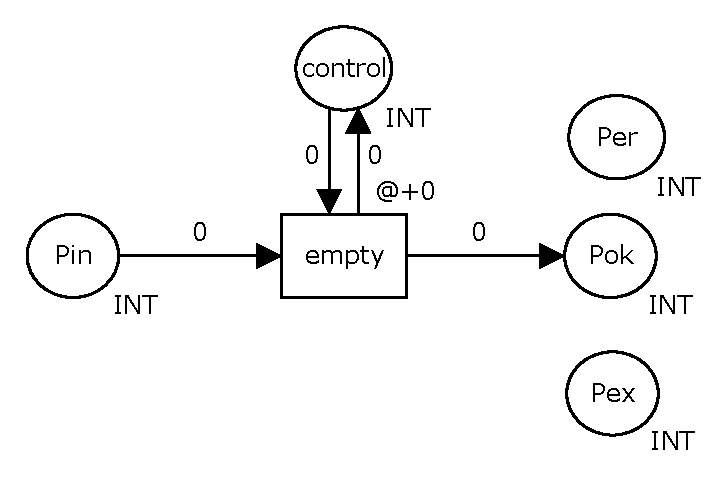
\includegraphics[width=0.45\textwidth]{Figures/empty.eps}
%    }
%    \hfill
%    \subfigure[First sub-figure\label{subfig-2:dummy}]{%
%      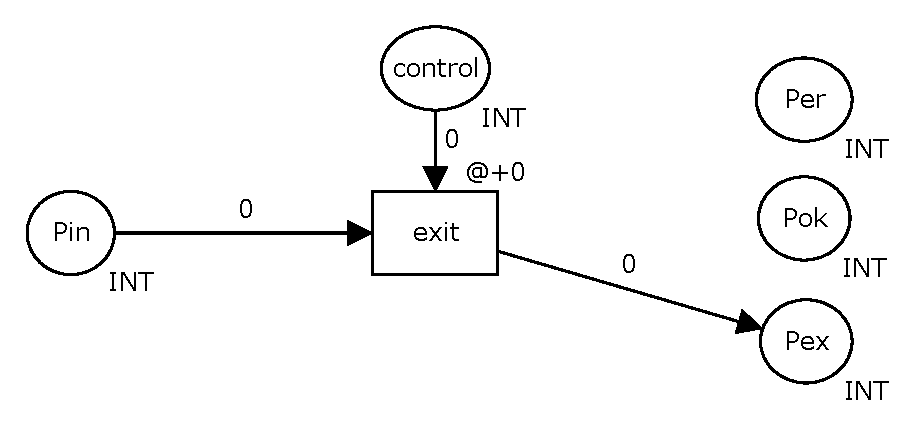
\includegraphics[width=0.45\textwidth]{Figures/exit.eps}
%    }
%    \caption{Dummy figure}
%    \label{fig:dummy}
%  \end{figure}
%  
%  \ref{subfig-1:dummy}
%and \ref{subfig-2:dummy}
%\section{Conclusions}\label{conclusions}1
%\markright{~\ref{conclusions} Conclusions}
%
%The work that has been carried out in this Thesis can be divided in two different topics: on the one hand the design and verification of Web Service compositions with time constraints by means of a top-down methodology called Correct-WS and the implementation of the WST tool supporting several phases of this methodology, and on the other hand the specification, validation and verification of electronic contracts with time constraints by means of the definition of a visual model with a formal background called \codiag.
%
%Concerning the first topic, the work carried out in \cite{Cambronero2007} has been continued and extended, adding things such as the treatment of exceptions. The WST tool has been improved in several aspects, completing the implementation of the translation from WS-CDL to timed automata and including the treatment of exceptions in all the different phases supported by the tool.
%
%The advantage of having the Correct-WS methodology and the WST tool is that the correctness of the Web Service compositions, with respect to some properties of interest, can be formally verified in the early phases of the development process. In this way, any problem detected can be solved before implementation, saving the cost of correcting these errors after implementation.
%Another important advantage is that we can obtain automatically XML code from a graphical model of the composition, so non-XML experts do not have to care about specifying the composition in languages such as WS-CDL.
%
%Regarding the second topic, a novel approach for the specification and verification of deontic e-contracts has been defined. It consists of a visual model called \codiag\ representing the obligations, permissions and prohibitions of the contract, including also any condition, reparation and time constraint. The syntax of the model has been formally defined, and the semantics is provided by means of a transformation into a network of timed automata, allowing the verification of some properties of interest on it by using the model-checker of the UPPAAL tool.
%
%Apart from the timed automata semantics, some other applications of \codiag\ are envisaged. They can be used as a user-friendly way of specifying a contract in \CL\ language, as a translation function from \codiag\ to \CL\ has been defined. The diagrams can also be used to check if the behaviours of systems, modelled as timed automata, comply with the contracts represented by \codiag. This can be done by applying the set of satisfaction rules that has been defined.
%
%The main advantage of \codiag\ is that they provide a graphical representation of e-contracts but amenable to formal verification. In this way, non-experts in formal methods can easily specify the contracts in a graphical manner and, as a formal semantics of the model has been defined, the specified contract can be formally verified with respect to some properties of interest. The formal verification of the e-contracts is important to find out any contradiction or unexpected behaviours allowed by the contract, so the contracts can be corrected in a suitable manner.
%
%\section{Contributions}\label{contributions}
%\markright{~\ref{contributions} Contributions}
%
%In this section the contributions produced as a result of the development of this Thesis are summarized in the following list:
%
%\begin{itemize}
%
%\item The continuation and extension of the development of the Correct-WS methodology for the design and verification of Web Service compositions.
%
%\item The improvement of the implementation of the WST tool that supports several phases of the Correct-WS methodology.
%
%\item The definition of a visual model called \codiag\ for the specification of deontic electronic contracts including time constraints.
%
%\item The definition of formal syntax and semantics for \codiag, allowing the formal verification of the contract modelled.
%
%\item The definition of a set of satisfaction rules to check the compliance of the contracts represented by \codiag.
%
%\item The definition of a translation function from \codiag\ to the contract language \CL.
%
%\end{itemize}
%
%\section{Future Works}\label{future}
%\markright{~\ref{future} Future Works}
%
%The work that has been presented in this Thesis has led to several ideas for future work. Some of them are the following:
%
%\begin{itemize}
%
%\item Concerning the WST tool, it is currently under development a new tab supporting the analysis phase of the Correct-WS methodology. This tab will allow the users to develop the KAOS model for the specification of the properties of interest, generating automatically the queries corresponding to this model that have to be check in the verifier of the UPPAAL tool. The inclusion of the translation of WS-CDL documents into Coloured Petri nets in the WST tool is also under development.
%
%\item A study of the complexity and scalability of \codiag\ to see how complex can be the electronic contracts that we can tackle with these diagrams.
%
%\item The application of \codiag\ to different contexts, such as requirements engineering (to formalize
%requirements), product software families (as an extension of feature diagrams), \ldots
%
%\item The development of a tool to model \codiag\ and automatizing the transformation of the diagrams into timed automata supported by the UPPAAL tool, in the same way that the WST tool automatizes several transformations of the Correct-WS methodology.
%
%\item The development of a query language for contracts making possible the specification at a high level of abstraction of the properties of the contracts we want to check, instead of specifying the properties directly in the query language used by the UPPAAL tool. Therefore, a correspondence between the contract query language and the UPPAAL query language would be necessary.
%
%\item We also envisage the possibility of specifying a different diagram for each one of the parties involved instead of having global \codiag\ with multiple agents. This compositional approach can be useful if a composition operator is defined, specifying when two of these new \codiag\ can be composed and the result of the composition.
%
%\end{itemize}
%
%\section{Publications and Collaborations}\label{publications}
%\markright{~\ref{publications} Publications}
%
%The work done during this Thesis has given rise to several publications. They include international journal papers, international conference papers, and a national conference paper. Two technical reports have also been published and works submitted for publication are mentioned too.
%
%\subsection{Journal Papers}
%
%\begin{itemize}
%
%\item 
%Cambronero, M.E., D\'iaz, G., Mart\'inez, E., Valero, V. and Tobarra, L. (2010).
%WST: A Tool Supporting Timed Composite Web Services Model Transformation, \emph{SIMULATION: Transactions of the Society for Modeling and Simulation International}.
%
%\item 
%Cambronero, M.E., D\'iaz, G., Valero, V. and Mart\'inez, E. (2011).
%Validation and Verification of Web Services Choreographies by Using Timed Automata, \emph{Journal of Logic and Algebraic Programming} \textbf{80} pp. 25-49.
%
%\item 
%Cambronero, M.E., Valero, V. and Mart\'inez, E.
%Design and Generation of Web Services Choreographies with Time Constraints, \emph{Journal of Universal Computer Science}, to appear in 2011.
%
%\end{itemize}
%
%\subsection{International Conference Papers}
%
%\begin{itemize}
%
%\item
%Cambronero, M.E., D\'iaz, G., Valero, V. and Mart\'inez, E. (2008). A Tool for the Design and Verification of Composite Web Services, in \emph{Second International Workshop on Formal Languages and Analysis of Contract-Oriented Software}, pp. 9-16.
%
%\item 
%Mart\'inez, E., D\'iaz, G., Cambronero, M.E. and Valero, V. (2009). Design and Verification of Web Services Compositions, in \emph{The Fourth International Conference on Internet and Web Applications and Services}, pp. 395-400.
%
%\item
%Valero, V., Macia, H. and Mart\'inez, E.(2009). Transforming WS-CDL specifications into Coloured Petri Nets, in \emph{International Workshop on Petri Nets and Software Engineering (PNSE09)}.
%
%\item
%Mart\'inez, E., D\'iaz, G., Mart\'inez, C.R., Cambronero, M.E. and Valero, V. (2009). Time Ordering Architecture in SCA, in \emph{TAMoCo 2009 Techniques and Applications for Mobile Commerce}, pp. 117-125.
%
%\item
%Cambronero, M.E., D\'iaz, G., Mart\'inez, E. and Valero, V. (2009). A comparative study between WSCI, WS-CDL, and OWL-S, in \emph{The 2009 IEEE International Conference on e-Business Engineering (ICEBE 2009)}, pp. 377-382.
%
%\item 
%Andr\'es, C., D\'iaz, G., Mart\'inez, E. and Zhang, Y (2009). Formal Study of Prioritized Service Compositions, in \emph{International conference on signal-image technology \& internet based systems, 5th (SITIS 2009)}, pp. 355-362.
%
%\item 
%Mateo, J.A., D\'iaz, G., Mart\'inez, E. and Cambronero, M.E. (2010). Modeling Conference Contribution Management Using Web Services, in \emph{The Fifth International Conference on Internet and Web Applications and Services}, pp. 463-468.
%
%\item
%Mart\'inez, E., D\'iaz, G., Cambronero, M.E. and Schneider, G. (2010). A Model for Visual Specification of e-Contracts, in \emph{The 7th IEEE International Conference on Services Computing (SCC 2010)}, pp. 1-8.
%
%\item
%Mart\'inez, E. and Schneider, G. (2010). Automated Analysis of Conflicts in Software Product Lines, in \emph{1st International Workshop on Formal Methods in Software Product Lines Engineering}, pp. 75-82.
%
%\item
%Mart\'inez, E., D\'iaz G. and Cambronero, M.E. (2010). Visual Specification of Formal e-Contracts, in \emph{Fourth Workshop on Formal Languages and Analysis of Contract-Oriented Software}, pp. 55-62.
%
%\item
%Mateo, J.A., Valero, V., Mart\'inez, E. and D\'iaz, G. (2011). Analysis and Verification of Web Services Resource Framework (WSRF) specifications Using Timed Automata Modeling Conference Contribution Management Using Web Services, in \emph{The Sixth International Conference on Internet and Web Applications and Services}, pp. 222-227.
%
%\item
%Mart\'inez, E., Cambronero, M.E., D\'iaz, G. and Schneider, G. (2011). Timed Automata Semantics for Visual e-Contracts, in \emph{Fifth Workshop on Formal Languages and Analysis of Contract-Oriented Software}, pp. 7-22.
%
%\item
%Mart\'inez, E., D\'iaz, G. and Cambronero, M.E. Contractually Compliant Service Compositions, \emph{The Ninth International Conference on Service Oriented Computing}, to appear in 2011.
%
%\end{itemize}
%
%\subsection{National Conference Papers}
%
%\begin{itemize}
%
%\item 
%Valero, V., Macia, H. and Mart\'inez, E.(2009). A Petri Net Semantics for WS-CDL, in \emph{XVII Jornadas de Concurrencia y Sistemas Distribuidos}, pp. 35-50.
%
%\end{itemize}
%
%\subsection{Technical Reports}
%
%\begin{itemize}
%
%\item Cambronero, M.E., Valero, V., D\'iaz, G. and Mart\'inez, E. (2009). Web Services Choreographies Verification, \emph{Technical Report DIAB-09-04-3}, Computing Systems Department, University of Castilla-La Mancha.
%
%\item Cambronero, M.E., D\'iaz, G., Mart\'inez, E. and Valero, V. (2009). A comparative study between WSCI, WS-CDL, and OWL-S, \emph{Technical Report DIAB-09-04-3}, Computing Systems Department, University of Castilla-La Mancha.
%
%\end{itemize}
%
%%\subsection{Submitted Works}
%
%\subsection{Collaborations}
%
%International Collaborations and stays at international universities and research groups:
%
%\begin{itemize}
%
%\item Department of Applied IT at Chalmers | University of Gothenburg - Sweden for 3 months in 2009.
%
%\end{itemize}
%
%\section{Funds and Grants}\label{funds}
%\markright{~\ref{funds} Funds and Grants}
%
%The present Thesis has been carried out thanks to the funds received from a number of projects and grants:
%
%\begin{itemize}
%
%\item Research project: Modelling and Analysis of Composed Web Services Using Formal Techniques (TIN2009-14312-C02-02)\newline
%Research project funded by Spanish Ministry of Education \& Science.\newline
%Participating Organizations: University de Castilla-La Mancha (Spain).
%
%\item The author of this thesis has been supported by a predoctoral grant from the \textit{Junta de Comunidades de Castilla-La Mancha}, as a part of the program ``\textit{Plan Regional de Investigaci\'{o}n Cient\'{\i}fica, Desarrollo Tecnol\'{o}gico e Innovaci\'{o}n 2005-2010 (PRINCET)}''.
%
%\end{itemize}